\documentclass[../Proposed Method.tex]{subfiles}
\begin{document}

% \textbf{What are sliding windows}
The time span of this research is 10 years, from 2012/01 to 2021/12. If we use only one trading strategy throughout such a long period of time, it will most likely to encounter an overfitting problem. Our trading strategy may not be the most profitable. To avoid this problem, the sliding window method is deployed. The sliding window consist of a training period and a testing period, and it slides according to the testing period up to the end of the investment period. Sliding window can reduce the amount of training data by splitting the training data into several different time frame. Each time frame is trained by GNQTS independently, thus the strategies that GNQTS finds will be better adapted to each period of time. To compare which time frame that GNQTS will find a better rate of return, we use 60 different sliding windows in this research.

\bigbreak

% \textbf{Old sliding sindows}
In xxx's research, 13 different sliding windows are indroduced, as shown in table \ref{sw}.

\begin{table}[H]
    \centering
    \captionsetup{font={footnotesize}}
    \caption{13 kinds of sliding windows}
    \label{sw}
    \footnotesize
    \begin{tabularx}{0.5\textwidth}{c @{\extracolsep{\fill}} cc}
        \toprule
        \textbf{Symmetric} & \textbf{Asymmetric} & \textbf{Year-on-year} \\
        \midrule
        M2M                & Q2M H2Q             & M*                    \\
        Q2Q                & H2M Y2Q             & Q*                    \\
        H2H                & Y2M Y2H             & H*                    \\
        Y2Y                &                     &                       \\
        \bottomrule
    \end{tabularx}
\end{table}

There are three types of sliding windows, symmetric, asymmetric and year-on-year.
The original sliding windows are composed of 4 types of time frame, month (M), quarter (Q), half year (H), and year (Y). The comination of these time frame determine the training period and testing period of a sliding window. As for year-on-year, the training period and testing period are one year apart, because of considering that the business cycle repeated every year for some certain industries. For example, M2M is a sliding window with one month of training period and one month of testing period. Figure \ref{M2M}, \ref{H2Q}, and \ref{H_star} demostrate the symmetric, asymmetric and year-on-year sliding window M2M, H2Q, and H* investing in 2010 and 2011.

\begin{figure}[H]
    \centering
    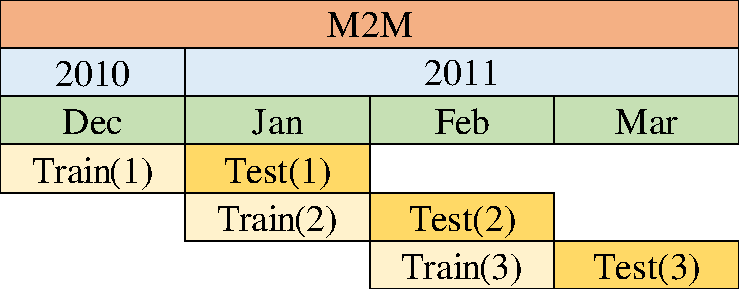
\includegraphics[scale = 0.5] {figure/M2M.pdf}
    \captionsetup{font={footnotesize}}
    \caption{Demonstration of M2M sliding window}
    \label{M2M}
\end{figure}

\begin{figure}[H]
    \centering
    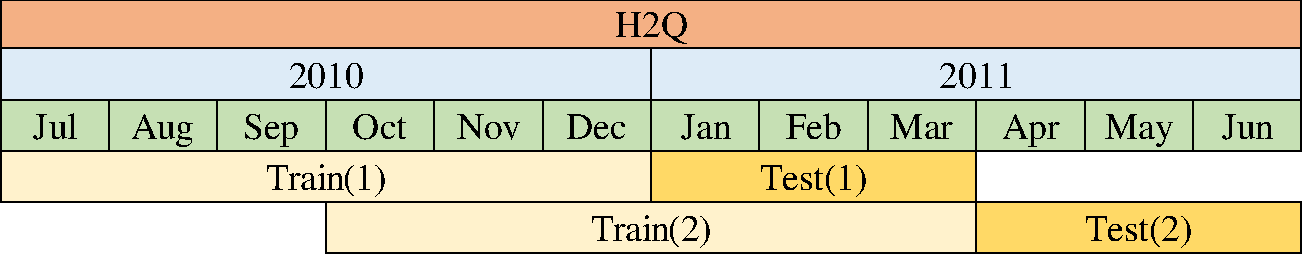
\includegraphics[scale = 0.5] {figure/H2Q.pdf}
    \captionsetup{font={footnotesize}}
    \caption{Demonstration of H2Q sliding window}
    \label{H2Q}
\end{figure}

\begin{figure}[H]
    \centering
    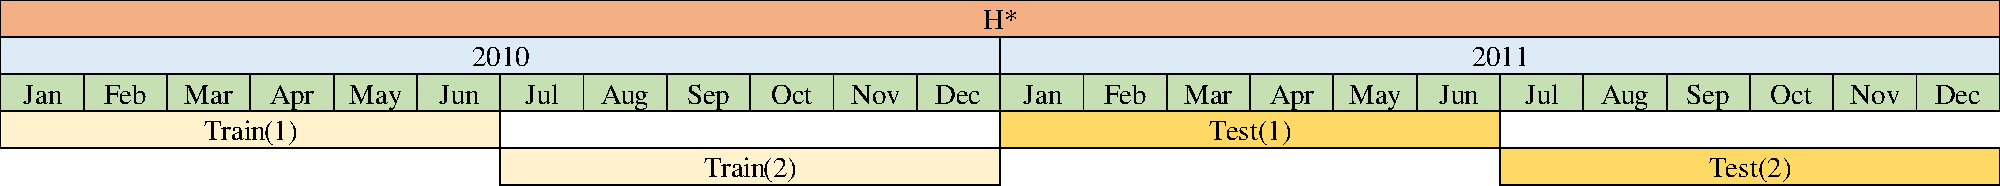
\includegraphics[scale = 0.5] {figure/H_star.pdf}
    \captionsetup{font={footnotesize}}
    \caption{Demonstration of H* sliding window}
    \label{H_star}
\end{figure}

% \textbf{New sliding windows}
To better understand the effect of different time period that apply to the sliding window. More time frames are introduced to the training period and testing period. These new times frames are days, weeks, one and a half year, two years, and three years. The newly created sliding windows are as shown in table \ref{new_sw}, where D stands for day, W stands for week, and M stands for month. For instance, 20D20 is a sliding window with 20 days of training period and 20 days of testing period.
%  With more sliding windows, 

\begin{table}[H]
    \centering
    \captionsetup{font={footnotesize}}
    \caption{new sliding windows}
    \label{new_sw}
    \footnotesize
    \begin{tabularx}{0.7\textwidth}{cc@{\extracolsep{\fill}}cccc}
        \toprule
        \multicolumn{2}{c}{\textbf{days}} & \textbf{weeks} & \textbf{one and a half year} & \textbf{two years} & \textbf{three years}         \\
        \midrule
        20D20                             & 5D5            & 4W4                          & 18M18              & 24M24                & 36M36 \\
        20D15                             & 5D4            & 4W3                          & 18M12              & 24M18                & 36M24 \\
        20D10                             & 5D3            & 4W2                          & 18M6               & 24M12                & 36M18 \\
        20D5                              & 5D2            & 4W1                          & 18M3               & 24M6                 & 36M12 \\
        15D15                             & 4D4            & 3W3                          & 18M1               & 24M3                 & 36M6  \\
        15D10                             & 4D3            & 3W2                          &                    & 24M1                 & 36M3  \\
        15D5                              & 4D2            & 3W1                          &                    &                      & 36M1  \\
        10D10                             & 3D3            & 2W2                          &                    &                      &       \\
        10D5                              & 3D2            & 2W1                          &                    &                      &       \\
                                          & 2D2            & 1W1                          &                    &                      &       \\
        \bottomrule
    \end{tabularx}
\end{table}

\end{document}